\subsection{Continuity of Finite Elements}
When designing finite elements, it can be easy to be seduced by the 
locality of each finite element, and forget to keep the original 
problem in mind. In this section we examine how different requirements 
on the solution can affect how the finite elements are constructed 
using different examples.
Say, to start, we only require the solution to be continuous, 
everywhere on $\OO$.
To do so, when the solution transitions from element to element, 
the solution must `match up', coming from each element. 
One way to include this in the construction can be seen in the 
following example.
\begin{exmp}{\quad\label{exmp:c0_triangle_con}}
For some $\OO$, let $\mathcal{T}$ be an admissible partition into 
triangles. 
Let $t >0$, and for each finite element, let $\Pi = \mathcal{P}_t$, resulting 
in finite elements with complete polynomials.
In each $T_i$ place
$s = (t+1)(t+2)/2$ points such that:
\begin{itemize}
    \item The points create a grid
    \item There are $t+1$ points on each edge of $T_i$
    \item Every point not on an edge is on an orthogonal intersection of lines drawn between points on the edges 
\end{itemize} 
An illustration of this can be seen in Figure~\ref{fig:triangle_nodal}, for 
$t=5$.
By choosing values for each point, every polynomial on each $T_i$ 
is uniquely determined (the proof of uniqueness can be found in~\cite{Braess}, page 64).
By restricting the polynomials to an edge, they become polynomials of 
one variable, and are uniquely determined by the values at the $t+1$ points 
on that edge.

Since the values and the points at each edge is the same, polynomials from 
neighbouring elements reduce to the same polynomial, and we get global 
continuity.
\end{exmp}
\begin{figure}[ht]
    \centering
    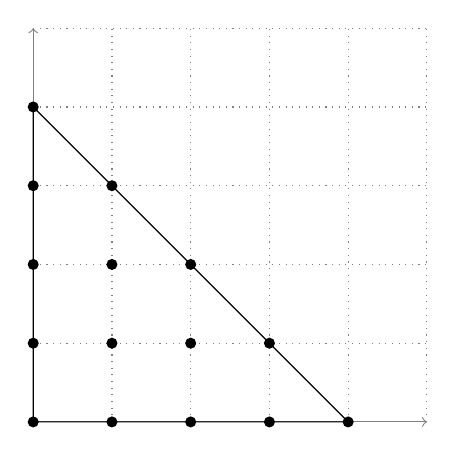
\begin{tikzpicture}
	\draw[color=gray,dotted] (0,0) grid (5,5);
	\draw[->, color=gray] (0,0) -- (5,0);
	\draw[->,color=gray] (0,0) -- (0,5);
	\draw[-,color=black] (0,0) -- (0,4) -- (4,0) --(0,0);
	\foreach \p in {(0,4),
			(0,3), (1,3),
			(0,2), (1,2), (2,2),
			(0,1), (1,1), (2,1), (3,1),
			(0,0), (1,0), (2,0), (3,0), (4,0)}
		\fill \p circle(2pt);
\end{tikzpicture}
    \caption{Triangle element, with nodes for $t=5$}\label{fig:triangle_nodal}
\end{figure}
Example~\ref{exmp:c0_triangle_con} demonstrates, that global continuity are 
somewhat easy to obtain, and constructing finite elements using polynomials 
of any degree grants this property. Letting $t=1$ results in finite elements 
where $\dim(\Pi_i)=3$, and finding the solution becomes computationally 
easy.

If, however, we search for solutions which 
are $C^1(\OO)$, difficulty increases. Along each edge the functions 
themselves must match up, but the first derivatives must now also match. 
We express this using the normal derivative, and showcase this in the 
following example. 
\begin{exmp}{\quad\label{exmp:c1_triangle_con}}
   As in Example~\ref{exmp:c0_triangle_con}, 
    for some $\OO$, let $\mathcal{T}$ be an admissible partition into 
    triangles, and let $\Pi_i = \mathcal{P}_5$ for each finite element.
    Remember that $\dim(\mathcal{P}_5) = 21$.
    Let the values of the derivatives at each vertice be given up 
    to the $2$nd order, as well as the value of the normal derivative at the 
    midpoint of each element.
    
    To ensure a solution in $C^1(\OO)$, 
    we now check the solution three ways; inside each element ($1$), 
    on the vertices ($2$), and on the edges ($3$).
    \iffalse
    we now check the solution three ways:
    \begin{enumerate}
        \item Inside each element
        \item On the vertices
        \item On the edges
    \end{enumerate} 
    \fi

    \textbf{1:} Inside each element, the solution is polynomial of degree $5$, 
    and therefore also $C^1(T_i)$.

    \textbf{2:} At each vertice there is $6$ derivatives up to order $2$, which 
    determines a polynomial of degree $5$ uniquely, and grants first 
    degree differentiablity.

    \textbf{3:} Along the edge, the polynomials reduce to $1$ variable, and the 
    normal derivative is a polynomial of degree $4$. Since it follows 
    the derivatives up to the first order at each end of the edge, and 
    the value is given at the midpoint, the normal derivative is uniquely 
    determined as well.

    Thus the normal derivative is continuous everywhere, resulting in a 
    solution in $C^1(\OO)$. This element is well known, and called 
    Argyris element.
\end{exmp}
As we can see from Example~\ref{exmp:c1_triangle_con}, by requiring a 
solution be differentiable, construction of finite elements and computation 
becomes harder. 

Many different types of finite elements exists, and can differ wildly in how they 
are constructed. In Example~\ref{exmp:c0_triangle_con} and~\ref{exmp:c1_triangle_con} 
the finite elements are constructed using a nodal system-specifying all elements of $\Pi$ 
uniquely through values at a number of points. However something like Hsieh–Clough–Tocher element 
is constructed by subdividing triangles into further triangles and using 
cubic polynomials.

These previous examples show how to construct finite elements `well'-as 
the solution we find obeys the requirement, namely either being $C^0(\OO)$ or 
$C^1(\OO)$. However elements can also be constructed badly, as we will 
show here. In rectangular elements we use a polynomial family with 
tensor products:
\begin{equation*}
    \mathcal{Q}_t = \{ f(x,y)= \sum_{0\leq i,k \leq t} c_{ik}x^i y^k \}.
\end{equation*}
In the following example we will show how constructing finite elements 
can go wrong.
\begin{exmp}{\quad\label{exmp:c0_square_bad}}
   For some $\OO$, let $\mathcal{T}$ be an admissible partition into 
   rectangles, and for every $T_i$ let $\Pi_i = \mathcal{Q}_1$. 
   Every function in $\Pi_i$ then has the form 
   \begin{equation*}
    f(x,y) = a + bx + cy + dxy.
   \end{equation*}
   By specifying the values at every vertice of the element, every 
   function in $\Pi_i$ is uniquely determined. 
   As neighbouring elements share two vertices and values, and every $f\in\Pi_i$
   restricted to an edge is a linear function, we are guaranteed global 
   continuity. However, 
    as seen in Figure~\ref{fig:quad_element_bad}, if the element is rotated 
   at $45^\circ$, the term $dxy$ disappears and global continuity are longer 
   guaranteed.

   This can of course be remedied by either choosing elements differently, 
   or an appropiate transformation of variables.
\end{exmp}
\begin{figure}[ht]
    \centering
    \begin{tikzpicture}
	\draw[->, color=gray] (-2,0) -- (2,0);
	\draw[->,color=gray] (0,-2) -- (0,2);
	\path[draw=black] (1,0) -- (0,1) -- (-1,0) -- (0,-1) -- (1,0);
\end{tikzpicture}
    \caption{A quadrilateral element at $45^\circ$ from the axis}\label{fig:quad_element_bad}
\end{figure}
As can be seen in Examples~\ref{exmp:c0_triangle_con},~\ref{exmp:c1_triangle_con}, 
and~\ref{exmp:c0_square_bad}, there are many different ways to construct 
finite elements, and doing so is not an exercise divorced %! ved ikke om jeg kan lide den her formulering, men nok mest fordi jeg ikke fatter den
from $\OO$ or 
the requirements on the solution. In this chapter we have looked at what FEM is practically, and how we construct 
meshes using different partitions, and how those partitions are created using 
finite elements. We now move on to examining how the error of using a 
FEM solution behaves.

%! Jeg kan ikke finde dokumentet som indeholder Theorem 4.10, i min pdf står der "theese"